% Inbuilt themes in beamer
\documentclass{beamer}

% Theme choice:
\usetheme{Berlin}
\usecolortheme{seahorse}

% packages
%\usepackage[hmargin=2cm, vmargin=2cm]{geometry}
\usepackage{microtype}
\usepackage{graphicx}
\usepackage{hyperref}
\usepackage[english]{babel}
\usepackage{setspace}
%\usepackage{xcolor}
\usepackage{multicol}
\usepackage{float}
\usepackage{amsmath}
\usepackage{amssymb}
\usepackage[font=small,skip=2pt]{caption}
\usepackage[
backend=biber,
style=authoryear-comp,
]{biblatex}

\addbibresource{../RMbibliography.bib}
\parindent=0pt

% Title page details: 
\title{Scalar on Function Regression}
\author{Jonathan Willnow, Jakob Juergens, Jonghun Baek}
\date{{\color{red}}Presentation Day}

\begin{document}
	
	% Title page frame
	\begin{frame}
		\titlepage 
	\end{frame}
	
	% Remove logo from the next slides
	\logo{}
	
	% I'm not really a fan of a table of contents in short presentations (Jakob)
	% Outline frame
	%\begin{frame}{Outline}
	%	\tableofcontents
	%\end{frame}
	
	\begin{frame}{Introduction}
		Jona \\	
		\begin{itemize}
			\item Near-infrared (NIR) spectroscopy enables fast diagnostics by using the NIR region of the electromagnetic spectrum
			\item Suited for field-monitoring / on-line analysis and diagnostics of e.g: prediction of octane ratings!
			
			\item Spectroscopy results in high-dimensional dataset.
			\item
			This set of measurements along a continuum can be viewed as set of smooth spectral curves
			\item
			Regression to determine relationship between octane rating and spectral curves
			\end{itemize}
	\end{frame}
	
	\begin{frame}{Theory}
		
		Motivation from multivariate regression (multivariate dgp).
		
		\begin{itemize}
			\item
			A simple functional dataset is given by $x_{n}(t_{j,n}) \in \mathbb{R}, t_{j,n} \in [T_1, T_2], n = 1,2,...,N, j = 1,2,..., J_n  $
			\item Continuous underlying process, where $x_n(t)$ exists at any point $t$, but is only observed at $x_{n}(t_{j,n})$
			\item NIR-spectroscopy measurements, financial data, medical data, human perception (musical pitch, ...)
			
			\item To abstract information from the curves, they must be interpretable!
			
			\end{itemize}
	\end{frame}

	\begin{frame}{Theory}
		Jonghun
		\begin{itemize}
			\item Random Functions (name square integrable functions)
			\item Motivate continuous stochastic processes (growth curves/electricity consumption/yield curves/stonks)
			\item Use curves to predict a scalar response (show typical dgp)
		\end{itemize}
	\end{frame}

	\begin{frame}{Theory}
		Jonghun
		\begin{itemize}
			\item Basis expansions (b-splines and fourier)
			\item Talk about purposes
			\item Plots and show bias variance tradeoff
		\end{itemize}
	\end{frame}

	\begin{frame}{Theory}
		Jakob
		\begin{itemize}
			\item Random function represented as linear combination of basis functions $\checkmark$
			\item Just transform to multiple linear regression setting $\checkmark$
			\item You already know that from the beginning $\checkmark$
		\end{itemize}
	\end{frame}

	\begin{frame}{Estimation via Basis Representation}
		Assume the following data generating process
		$$Y(\omega) = \alpha + \int_{0}^{1} \beta(s) F(\omega)(s) \mathrm{d}s + \epsilon(\omega)$$
		\begin{itemize}
			\item $Y$ and $\epsilon$ realize in $\mathbb{R}$ and $F$ realizes in $\mathbb{L}^2[0,1]$
		\end{itemize}
		\vspace{0.2cm}
		
		Assume that we have a data set containing observations each of which is made up of:
		\begin{itemize}
			\item $y_i$: a scalar realization of $Y$
			\item $f_i(t)$: a realization of $F$
		\end{itemize}

	\end{frame}

	\begin{frame}{Estimation via Basis Representation}
		Let $\{b_i(t) \: \vert \: i = 1, \dots, \infty\}$ be a basis of $\mathbb{L}^2[0,1]$
		\vspace{0.2cm}
		
		Then we have the following representation of $\beta(t)$
		$$\beta(t) = \sum_{j = 1}^{\infty} \psi_j b_j(t) = \sum_{j = 1}^{L} \psi_j b_j(t) + \delta(t) \approx \sum_{j = 1}^{L} \psi_j b_j(t)$$
		and we can transform the data generating process into:
		\begin{equation}\notag
			\begin{split}
				Y(\omega) & = \alpha + \int_{0}^{1}\left[\left(\sum_{j = 1}^{\infty} \psi_j  b_j(s)\right) F(\omega)(s) \right]\mathrm{d}s + \epsilon(\omega) \\
						  & = \alpha + \sum_{j = 1}^{\infty} \left[\psi_j \textcolor{red}{\int_{0}^{1} F(\omega)(s) b_j(s)\mathrm{d}s}\right] + \epsilon(\omega)	  
			\end{split}
		\end{equation}
	\end{frame}

	\begin{frame}{Estimation via Basis Representation}
		$$Z_j(\omega) = \int_{0}^{1} F(\omega)(s) b_j(s)\mathrm{d}s$$ 
		This is a scalar random variable leading to the following transformation
		$$Y(\omega) = \alpha + \sum_{j = 1}^{\infty} \psi_j Z_j(\omega) + \epsilon(\omega)$$
		Each combination of observation $f_i(t)$ and deterministic basis function $b_j(t)$ effectively gives us a realization of this random variable.
		$$Z_{i,j} = \int_{0}^{1} f_i(s) b_j(s)\mathrm{d}s$$
		
	\end{frame}

	\begin{frame}{Estimation via Basis Representation}
		This allows us to write each observation in the data set as
		\begin{itemize}
			\item $y_i$: a scalar realization of $Y$
			\item $\left(Z_{i,j}\right)_{j \in \mathbb{N}}$: a countably infinite sequence of scalars
		\end{itemize}
		\vspace{0.2cm}
		
		Truncating the functional basis allows us to approximate the data set in the usual multivariate form.
		\begin{itemize}
			\item $y_i$: a scalar realization of $Y$
			\item $\left(Z_{i,1} \: \dots \:  Z_{i,L} \right)'$: a vector of scalar regressors
		\end{itemize}
		\vspace{0.2cm}
		
		Coefficients can then be estimated using theory from multivariate regression leading to an estimated coefficient vector $\hat{\beta}_L \in \mathbb{R}^L$.
	\end{frame}

	\begin{frame}{Estimation via Basis Representation}
		This can then be translated into an estimated coefficient function $\hat{\beta}(t)$ via:
	\end{frame}

	\begin{frame}{Theory - FPCA}
		Jakob
		\begin{itemize}
			\item Let's assume you know the theory of PCA (pc from varcov matrix) $\checkmark$
			\item Introduce mean and covariance functions of random functions $\checkmark$
			\item There is another cool basis $\rightarrow$ Eigenbasis (Karhunen-Loeve Expansion) $\checkmark$
			\item Sample Analog! (create a basis from observations and use for basis regression) $\checkmark$
			\item Plot fpcs and approximation of function realization
		\end{itemize}
	\end{frame}

	\begin{frame}{Spectral Representation of Random Vectors}
		Let $X(\omega)$ be a random vector realizing in $\mathbb{R}^p$.

		\begin{itemize}
			\item Let $\mu_x = \mathbb{E}(X)$ and $\Sigma_X = Cov(X)$
			\item Let $\{\gamma_i \: \vert \: i = 1, \dots, p\}$ be the orthonormal \textbf{Eigenvectors} of $\Sigma_X$
			\item Let $\{\lambda_i \: \vert \: i = 1, \dots, p\}$ be the corresponding \textbf{Eigenvalues} of $\Sigma_X$
		\end{itemize}
	
		\vspace{0.2cm}
		Then $X$ can also be represented as
		$$X(\omega) = \mu_x + \sum_{i = 1}^{p} \xi_i(\omega) \gamma_i$$
		where the $\xi_i(\omega)$ have the following properties
		
		\begin{multicols}{2}
			\begin{enumerate}
				\item $\mathbb{E}[\xi_i(\omega)] = 0$
				\item $Var(\xi_i(\omega)) = \lambda_i$
				\item $Cov(\xi_i(\omega), \xi_j(\omega)) = 0$ for $i \neq j$
			\end{enumerate}
		\end{multicols}
	\end{frame}

	\begin{frame}{Karhunen-Lo\'{e}ve Expansion}
		
		\textbf{Mean Function}: $$\mu(t) = \mathbb{E}\left[ F(\omega)(t) \right]$$

		\textbf{Autocovariance Function}: $$c(t,s) = \mathbb{E}\big[ \left( F(\omega)(t) - \mu(t) \right) \left( F(\omega)(s) - \mu(s) \right) \big]$$
		
		The \textbf{Eigenvalues} and \textbf{Eigenfunctions}: $\{(\lambda_i, \nu_i) \: \vert \: i \in \mathcal{I}\}$  are solutions of the following equation:
		$$ \int_{0}^{1}c(t,s)\nu(s) \mathrm{d}s = \lambda \nu(t) $$
	\end{frame}
	
	\begin{frame}{Karhunen-Lo\'{e}ve Expansion}
		A random function $F$ can be expressed in terms of its mean function and its Eigenfunctions:
		$$F(\omega)(t) = \mu(t) + \sum_{j = 1}^{\infty} \xi_j(\omega) \nu_j(t)$$
		
		Where the $\xi_j$ are scalar-valued random variables with the following properties.
		\begin{multicols}{2}
			\begin{enumerate}
				\item $\mathbb{E}[\xi_i(\omega)] = 0$
				\item $Var(\xi_i(\omega)) = \lambda_i$
				\item $Cov(\xi_i(\omega), \xi_j(\omega)) = 0$ for $i \neq j$
			\end{enumerate}
		\end{multicols}
		
		This representation is called the \textbf{Karhunen-Lo\'{e}ve Expansion} of the random function $F$ and the Eigenfunctions can serve as a basis to represent the function.
	\end{frame}

	\begin{frame}{Principal Component Analysis}
		A related concept is \textbf{Principal Component Analysis} (PCA).
		\vspace{0.2cm}
		
		$\Sigma_X$ unknown $\rightarrow$ \textbf{sample analogues}
	
		\begin{itemize}
			\item Let $\mathbf{X} \in \mathbb{R}^{n \times p}$ contain the standardized regressors
			\item Let $\hat{\Sigma}_X = \frac{\mathbf{X}'\mathbf{X}}{n}$
			\item Let $\{\hat{\gamma}_i \: \vert \: i = 1, \dots, p\}$ be the orthonormal \textbf{Eigenvectors} of $\hat{\Sigma}_X$
			\item Let $\{\hat{\lambda}_i \: \vert \: i = 1, \dots, p\}$ be the corresponding \textbf{Eigenvalues} of $\hat{\Sigma}_X$
		\end{itemize}
		\vspace{0.2cm} 
		
		Then $Z_i(\omega) = \hat{\gamma}_i' X(\omega)$ is called the i'th principal component and
		\begin{multicols}{2}
			\begin{enumerate}
				\item $\mathbb{E}[Z_i(\omega)] = 0$
				\item $Var(Z_i(\omega)) = \hat{\lambda}_i$
				\item $Cov(Z_i(\omega), Z_j(\omega)) = 0$ for $i \neq j$
			\end{enumerate}
		\end{multicols}
	\end{frame}

	\begin{frame}{Functional Principal Component Analysis}
		This idea can be extended to functional regressors in the form of \textbf{Functional Principal Component Analysis} (FPCA).
		\vspace{0.2cm}
		
		\textbf{Empirical Mean Function}:
		$$\hat{\mu}(t) = \frac{1}{n}\sum_{j = 1}^{n}f_j(t)$$

		\textbf{Empirical Autocovariance Function}:
		$$\hat{c}(t,s) = \frac{1}{n} \sum_{j = 1}^{n} \left(f_j(t) - \hat{\mu}(t)\right) \left(f_j(s) - \hat{\mu}(s)\right)$$

	\end{frame}

	\begin{frame}{Functional Principal Component Analysis}
	
		The \textbf{Eigenvalues} and \textbf{Eigenfunctions}: $\{(\hat{\lambda}_i, \hat{\nu}_i) \: \vert \: i \in \mathcal{I}\}$  are solutions of the following equation:
		$$ \int_{0}^{1}\hat{c}(t,s)\hat{\nu}(s) \mathrm{d}s = \hat{\lambda} \hat{\nu}(t) $$
		\vspace{0.2cm}
		
		The $\{\hat{\nu}_i(s) \: \vert \: i \in \mathcal{I}\}$ are called \textbf{Functional Principal Components} and can serve as a basis for representing the original curves. 
		\vspace{0.2cm}
		
		The corresponding scores $\hat{\xi}_i$ can be derived as
		$$\hat{\xi}_j(\omega) = \int_{0}^{1} (F(\omega)(s) - \hat{\mu}(s)) \hat{\nu}_j(s) \mathrm{d}s$$
		
	\end{frame}

	\begin{frame}{FPCA - Plots}
		\begin{minipage}[t]{0.79\textwidth}
			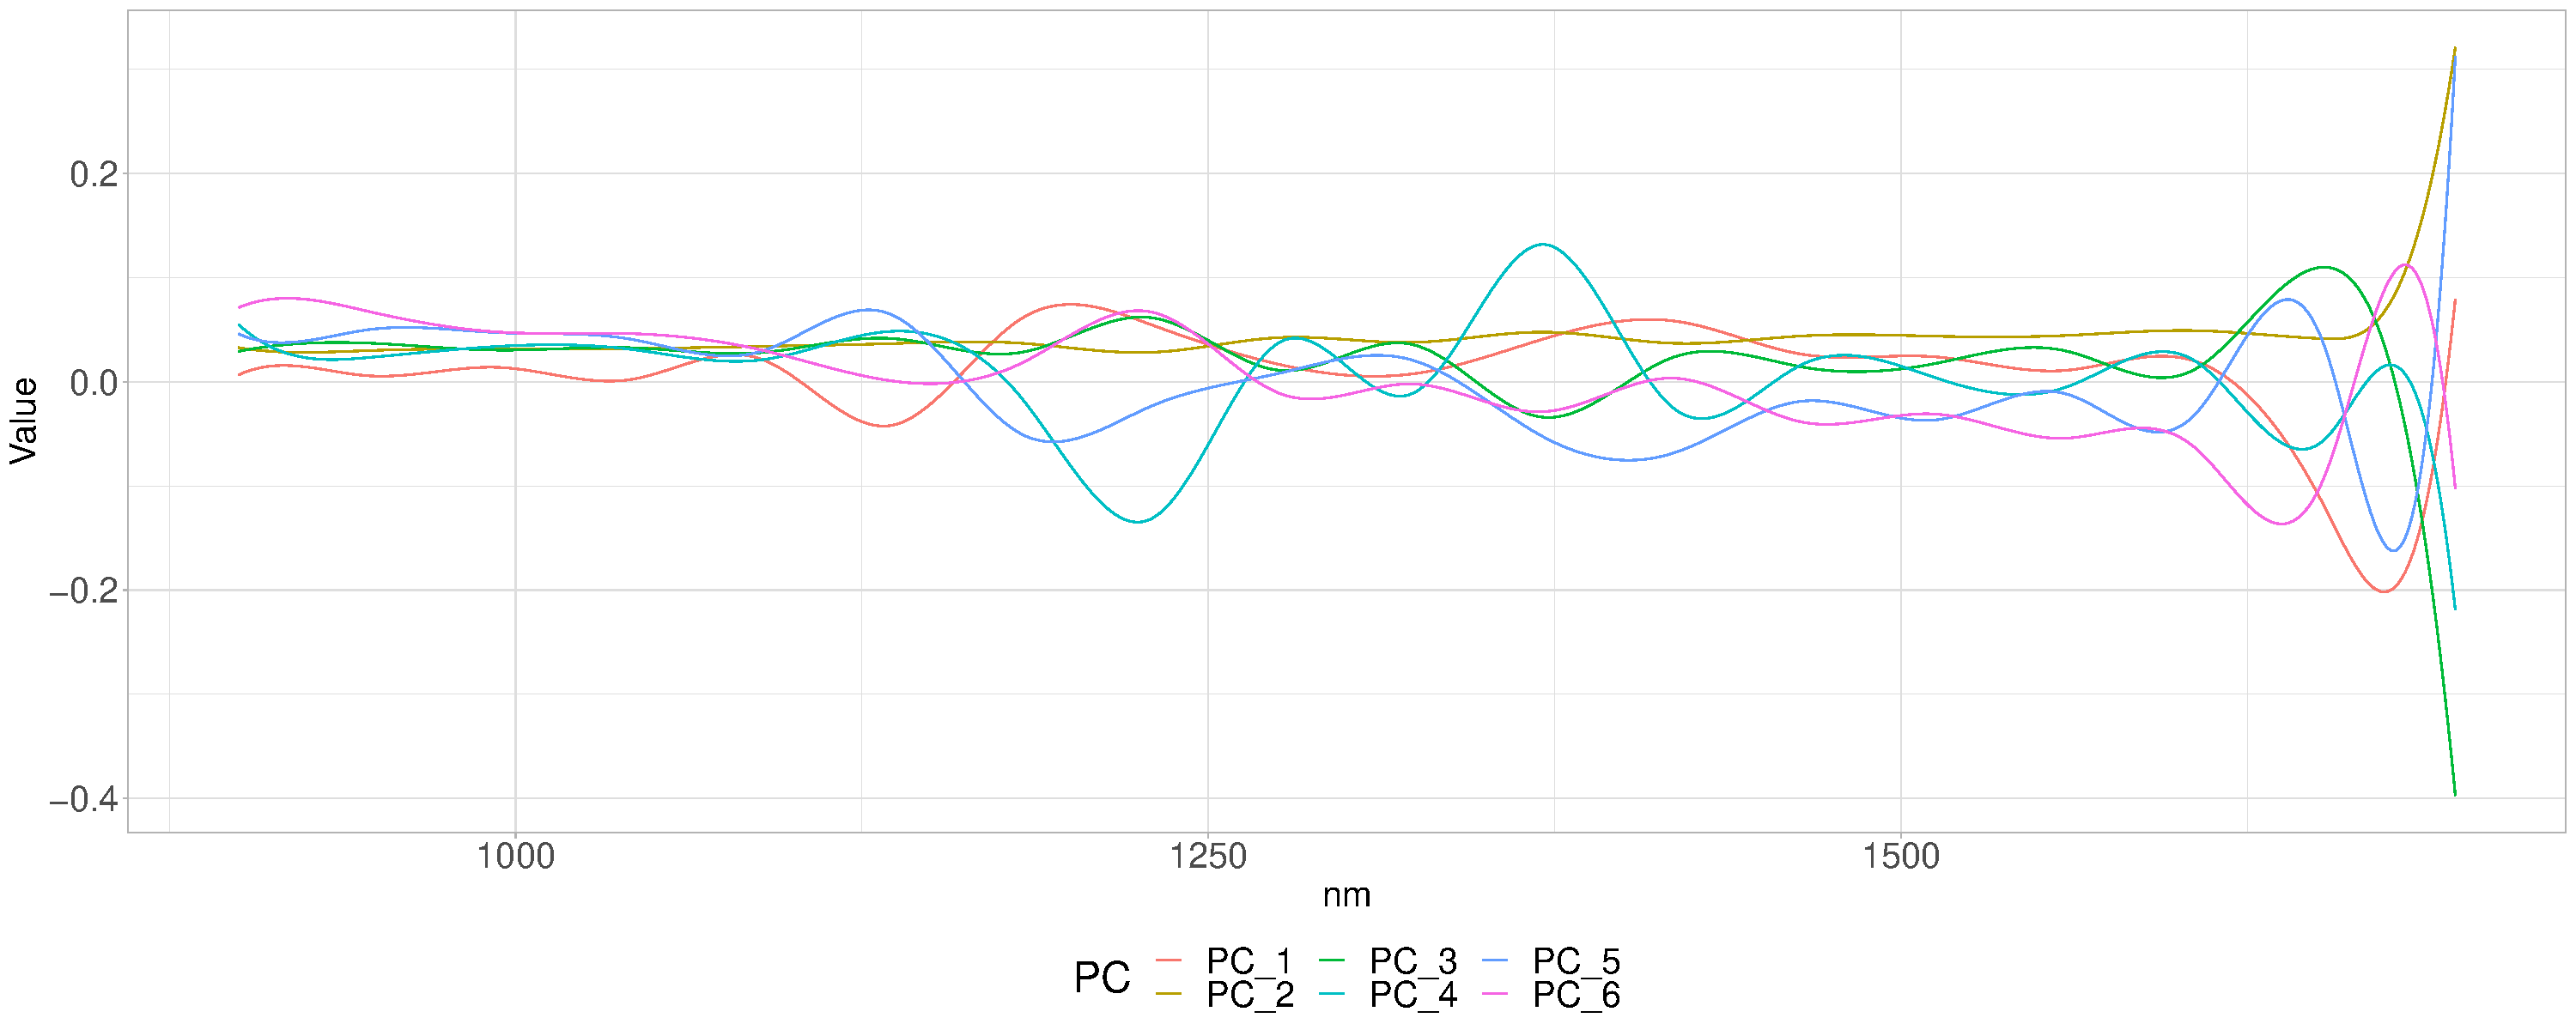
\includegraphics[width = \textwidth]{../Graphics/principal_components.pdf}
			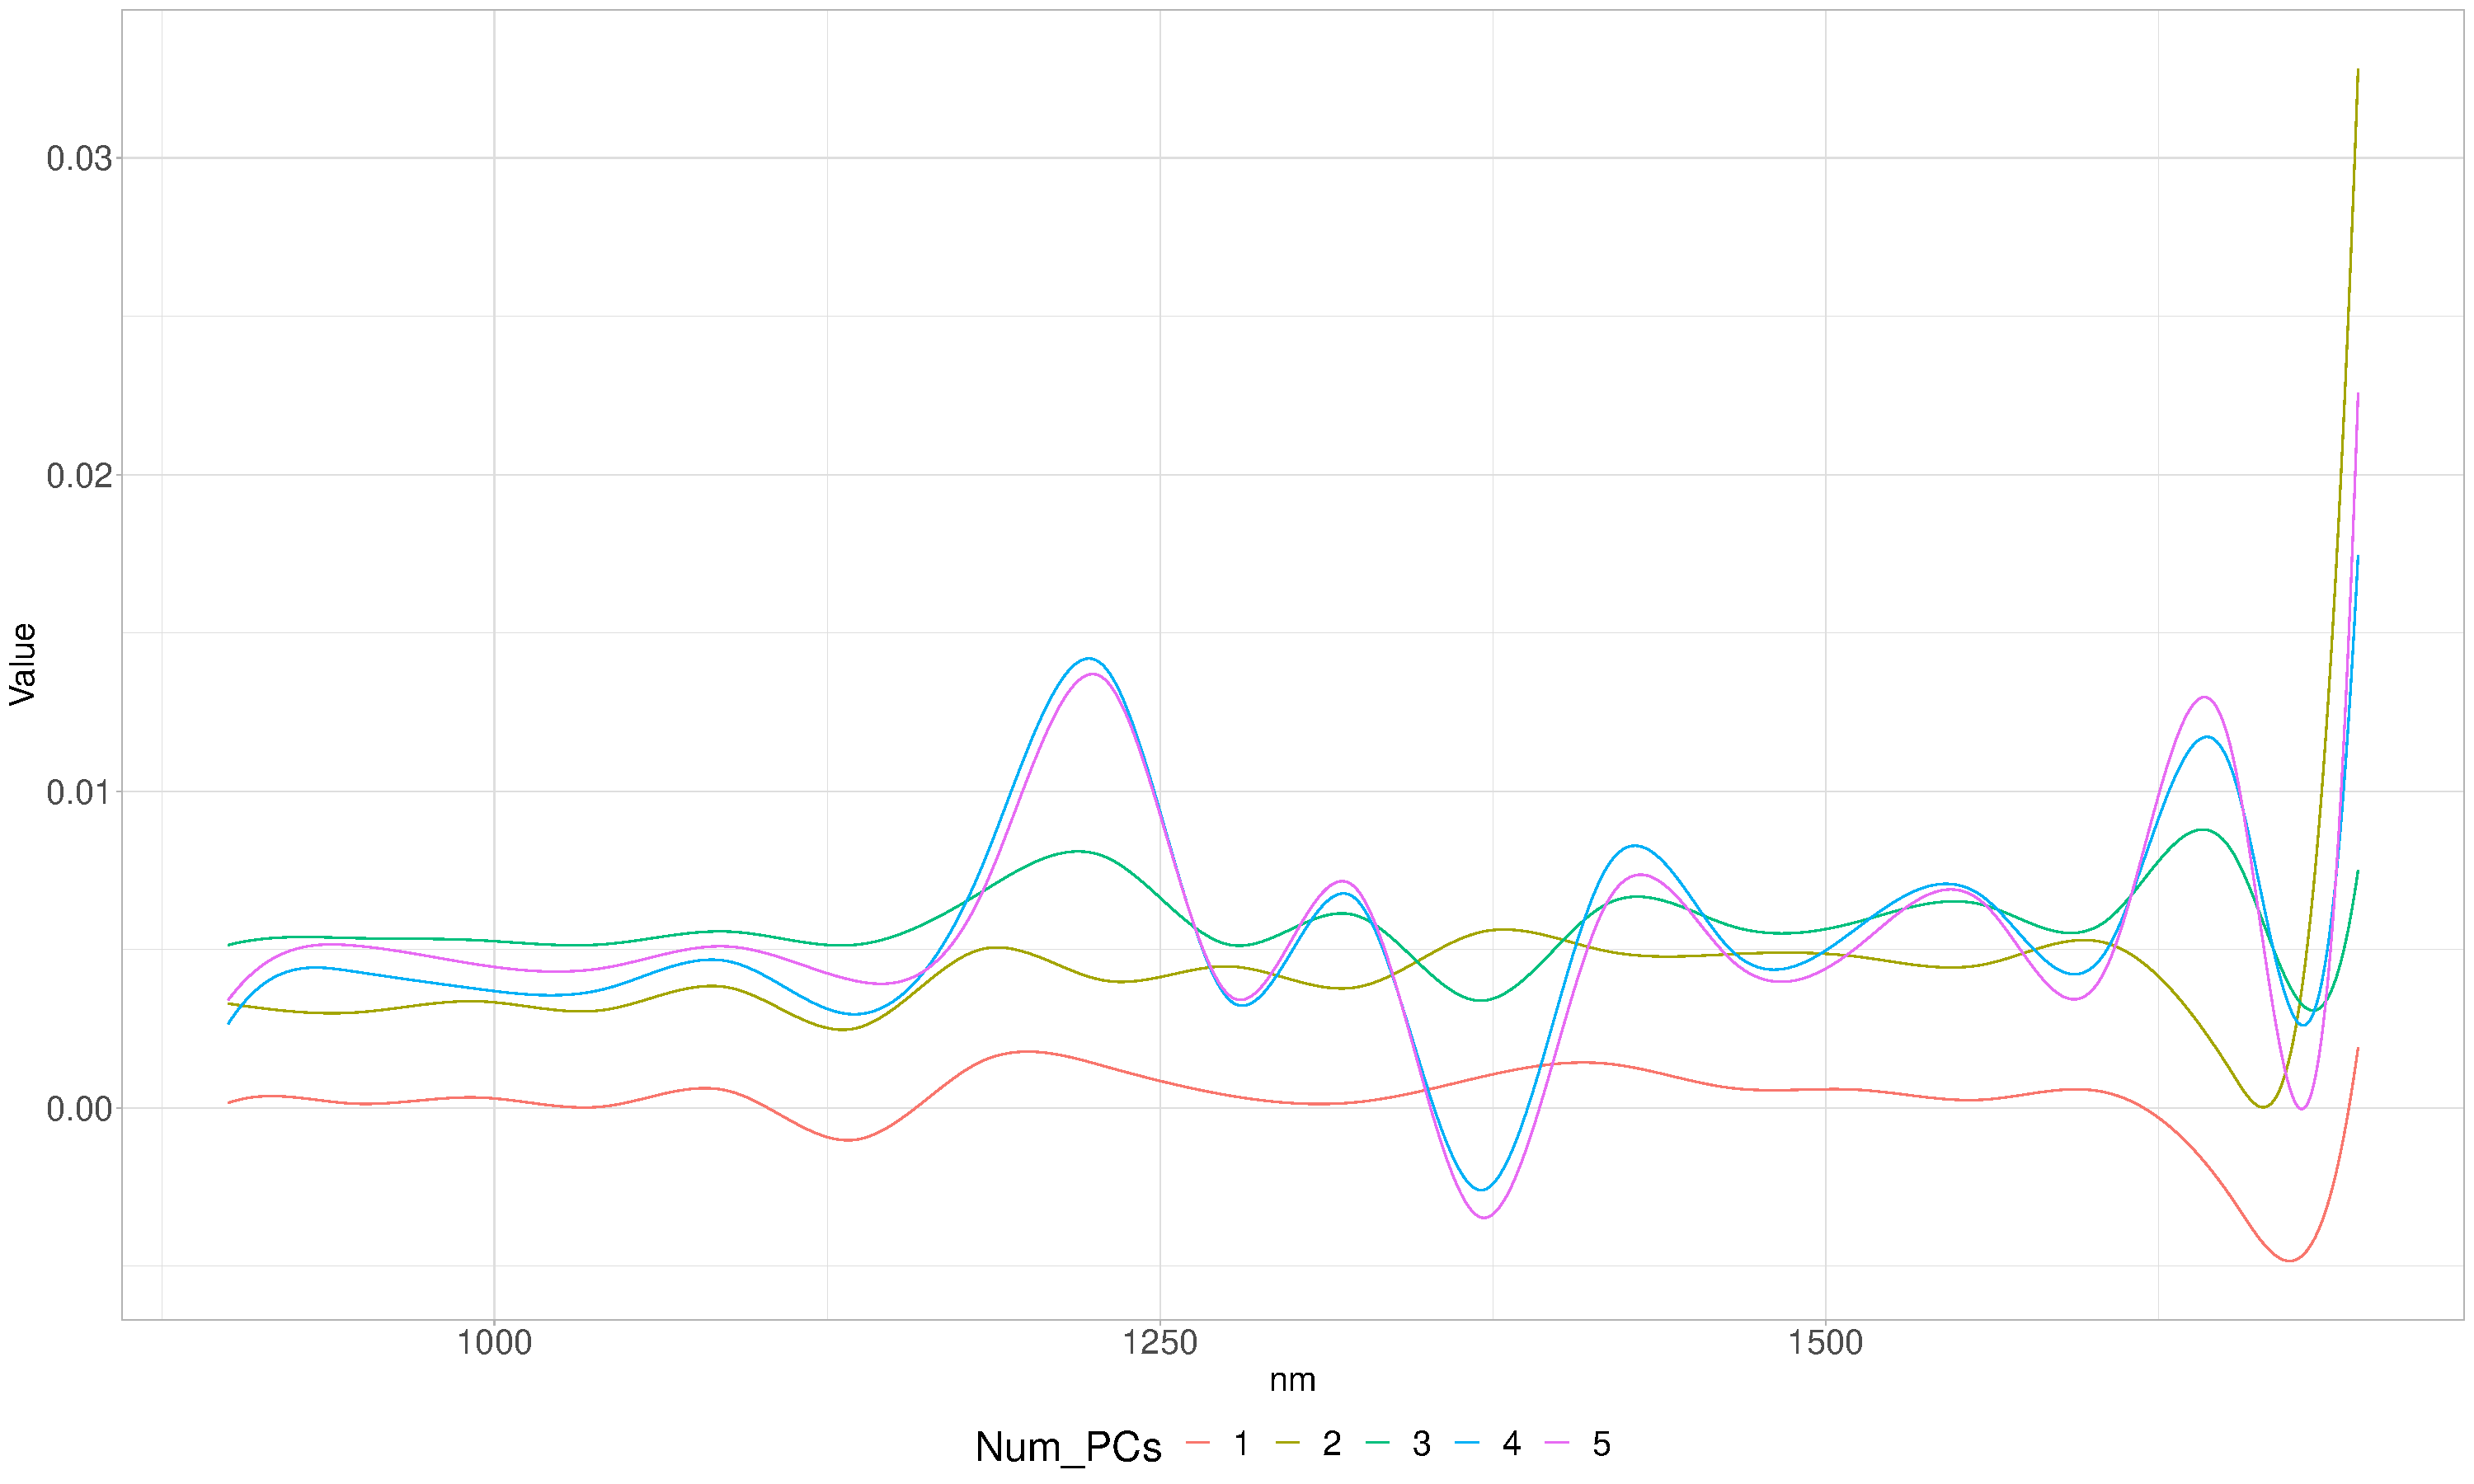
\includegraphics[width = \textwidth]{../Graphics/pc_approx.pdf}
		\end{minipage}
		\begin{minipage}[t]{0.19\textwidth}
			Lorem Ipsum Dolor Sit Amet
		\end{minipage}
	\end{frame}
	

	\begin{frame}{Simulation Setup \& Application}
		\begin{itemize}
		\item
		 Use the gasoline dataset (NIR-spectroscopy, 60 $\times$ 401) to predict octane ratings.
		\item 
		Generate new curves from gasoline dataset, motivated by Karhunen-Loeve expansion:
		
		$$F^{new}(\omega)(t) = \mu^{NIR}(t) + \sum_{j = 1}^{\infty} \xi_j^{new} \nu_j(t)^{new}$$ \\
		where \\
		 \vspace{0.1cm}
		$$\xi_{j}^{new} \in  \mathcal{N}_{n}(0,\Sigma)$$ \\
		and $\nu_j(t)^{new}$ be a $grid \times n_{FPC}$ matrix.
		
    		
		\end{itemize}
	\end{frame}
	
	
	\begin{frame}{Simulation Setup \& Application cont.}
		\begin{itemize}
		\item
		Following Reiss and Ogden (2007), let $f_1$ and $f_2$ be two true coefficient functions that differ in smoothness: 
		\vspace{0.4cm}
	

   $f_1 = 2\sin(0.5\pi t) + 4\sin(1.5 \pi t) + 5\sin(2.5 \pi t)$\\
   \vspace{0.1cm}
   

    
    $	f_2 = 1.5^{\frac{-0,5(t-0.3)^2}{0.02^2}} - 4^{\frac{-0,5(t-0.45)^2}{0.015^2}} +  8^{\frac{-0,5(t-0.6)^2}{0.02^2}} -  1^{\frac{-0,5(t-0.8)^2}{0.03^2}}$
   
    		
		\end{itemize}
		\vspace{0.1cm}
		\begin{figure}
\centering
\begin{minipage}{.5\textwidth}
  \centering
  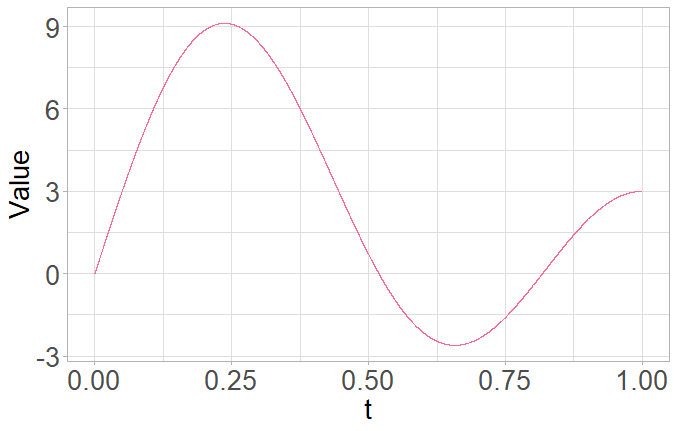
\includegraphics[height=3cm]{smooth_function.png}
  \captionof{figure}{$f_1$, smooth function}
  \label{fig:test1}
\end{minipage}%
\begin{minipage}{.5\textwidth}
  \centering
  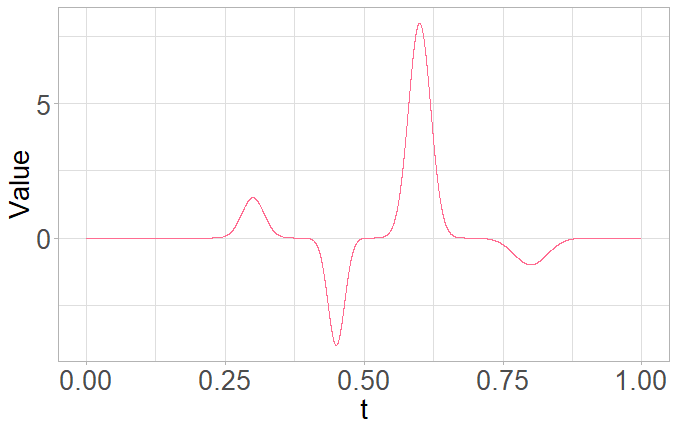
\includegraphics[height=3cm]{bumpy_function.png}
  \captionof{figure}{$f_2$, bumpy function}
  \label{fig:test2}
\end{minipage}
\end{figure}
		
	\end{frame}	

	
	\begin{frame}{Simulation Setup \& Application cont.}
		\begin{itemize}
		\item
    		Let \\
    		 \vspace{0.1cm}
    		
    		$Y_{1,f} = NIR \times f + \mathcal{N}(0,1) \times var(NIR \times f)/0.9 - var(NIR \times f)$, \\
    		  $Y_{2,f} = NIR \times f + \mathcal{N}(0,1) \times var(NIR \times f)/0.9 - var(NIR \times f)$ be two responses for $f \in f_1, f_2$.		
    		 	\item
    		 	 Four combinations with different number of cubic basis-function $n_{basis} \in (5,6,...,25)$ to perform regression using basis expansion and the FPCR approach.
			\item Compare results via criteria (CV, Mallows CP,...)
			\item 
			{\color{green} add results here!}
			
    		
		\end{itemize}
	\end{frame}
	
	
	\begin{frame}{Simulation Setup \& Application cont.}
		\begin{itemize}
		\item
    		Use insights from the simulation study to uncover dependence.
    		\item
    		Same setup, but without generated curves.
    		\item
    		Validation set approach:	Scores of testdata needs to be estimated by the trainingdata.  {\color{green} explain in detail?}
    		\item
    		Report results by MSE scaled by variance.
		\end{itemize}
	\end{frame}
	
	

	\begin{frame}{Summary}
		Jona \\
		Just summarize what we have done...
	\end{frame}

	\begin{frame}{further reading}
		Put footnotes here!
	\end{frame}
	
\end{document}